% !TEX program = xelatex

\documentclass[crop,tikz]{standalone}

\usepackage{amsmath}
\usepackage{fontspec}
\setmainfont{CMU Serif}

\usepackage{pgfplots}
\usepgfplotslibrary{fillbetween}

\usetikzlibrary{arrows.meta}
\usetikzlibrary{calc,patterns,angles,quotes}

\pgfdeclarelayer{background}
\pgfdeclarelayer{foreground}
\pgfsetlayers{background,foreground}

\pgfdeclarepatternformonly{my crosshatch dots}{\pgfqpoint{-2pt}{-1pt}}{\pgfqpoint{5pt}{5pt}}{\pgfqpoint{11pt}{10pt}}%
{
  \pgfpathcircle{\pgfqpoint{-1pt}{0pt}}{.5pt}
  \pgfpathcircle{\pgfqpoint{4pt}{3pt}}{.5pt}
  \pgfusepath{fill}
}

\tikzset{
  receiver/.pic={
    code={
      \coordinate (pole_left_bottom) at (0,0);
      \coordinate (pole_right_bottom) at ($ (pole_left_bottom) + (0.13,0) $);
      \coordinate (pole_left_top) at ($ (pole_left_bottom) + (0,2) $);
      \coordinate (pole_right_top) at ($ (pole_right_bottom) + (0,2) $);
      
      \draw[fill=white]
        (pole_left_top)
        --
        (pole_left_bottom)
        to[out=-45,in=-135,looseness=0.8]
        (pole_right_bottom)
        --
        (pole_right_top);
      
      \coordinate (rs_core_1) at ($ (pole_left_top) + (-0.22,0) $);
      \coordinate (rs_core_2) at ($ (rs_core_1) + (0.35,-0.08) $);
      \coordinate (rs_core_3) at ($ (rs_core_2) + (0.1,0.02) $);
      \coordinate (rs_core_4) at ($ (rs_core_3) + (0.15,0.12) $);
      \coordinate (rs_side_1) at ($ (rs_core_1) + (-0.03,0.1) $);
      \coordinate (rs_side_2) at ($ (rs_core_2) + (-0.02,0.1) $);
      \coordinate (rs_side_3) at ($ (rs_core_3) + (0.025,0.11) $);
      \coordinate (rs_side_4) at ($ (rs_core_4) + (0.02,0.095) $);
      \coordinate (rs_upper_1) at ($ (rs_side_1) + (-0.085,0.15) $);
      \coordinate (rs_upper_0) at ($ (rs_upper_1) + (-0.01,0.05) $);
      \coordinate (rs_upper_2) at ($ (rs_side_2) + (0.02,0.14) $);
      \coordinate (rs_upper_3) at ($ (rs_side_3) + (0.027,0.14) $);
      \coordinate (rs_upper_4) at ($ (rs_side_4) + (0.03,0.12) $);
      \coordinate (rs_top_1) at ($ (rs_upper_1) + (0.1,0.12) $);
      \coordinate (rs_top_0) at ($ (rs_top_1) + (-0.007,0.02) $);
      \coordinate (rs_top_2) at ($ (rs_upper_2) + (-0.03,0.15) $);
      \coordinate (rs_top_3) at ($ (rs_upper_3) + (-0.07,0.14) $);
      \coordinate (rs_top_4) at ($ (rs_upper_4) + (-0.09,0.105) $);
      \coordinate (rs_top_5) at ($ (rs_top_4) + (-0.03,0.02) $);
      \coordinate (rs_top_6) at ($ (rs_top_5) + (-0.3,0.035) $);
      \coordinate (rs_top_7) at ($ (rs_top_6) + (-0.1,-0.005) $);
      
      \draw[fill=white]
        (rs_core_1) -- (rs_core_2) -- (rs_core_3) -- (rs_core_4);
      
      \draw[fill=white]
        (rs_core_1) -- (rs_side_1) -- (rs_side_2) -- (rs_core_2) -- (rs_core_1);
      
      \draw[fill=white]
        (rs_core_2) -- (rs_side_2) -- (rs_side_3) -- (rs_core_3) -- (rs_core_2);
      
      \draw[fill=white]
        (rs_core_3) -- (rs_side_3) -- (rs_side_4) -- (rs_core_4) -- (rs_core_3);
      
      \draw[fill=white]
        (rs_side_1) -- (rs_upper_1) -- (rs_upper_2) -- (rs_side_2) -- (rs_side_1);
      
      \draw[fill=white]
        (rs_side_2) -- (rs_upper_2) -- (rs_upper_3) -- (rs_side_3) -- (rs_side_2);
      
      \draw[fill=white]
        (rs_side_3) -- (rs_upper_3) -- (rs_upper_4) -- (rs_side_4) -- (rs_side_3);
      
      \draw
        (rs_upper_1) -- (rs_upper_0);
      
      \draw[fill=white]
        (rs_upper_0) -- (rs_top_0) -- (rs_top_1) -- (rs_upper_1) -- (rs_upper_0);
      
      \draw[fill=white]
        (rs_upper_1) -- (rs_top_1) -- (rs_top_2) -- (rs_upper_2) -- (rs_upper_1);
      
      \draw[fill=white]
        (rs_upper_2) -- (rs_top_2) -- (rs_top_3) -- (rs_upper_3) -- (rs_upper_2);
      
      \draw[fill=white]
        (rs_upper_3) -- (rs_top_3) -- (rs_top_4) -- (rs_upper_4) -- (rs_upper_3);
      
      \draw[fill=white]
        (rs_top_0) -- (rs_top_1) -- (rs_top_2) -- (rs_top_3) -- (rs_top_4) --
        (rs_top_5) -- (rs_top_6) -- (rs_top_7) -- (rs_top_0);
    }
  }
}


\tikzset{
  satellite/.pic={
    code={
      \coordinate (center) at (0,0);
      
      % Right wing
      \coordinate (rw_top_right) at ($ (center) + (2,2.4) $);
      \coordinate (rw_bottom_right) at ($ (center) + (1.6,-2) $);
      \coordinate (rw_top_left) at ($ (center) + (0.47,2.3) $);
      \coordinate (rw_bottom_left) at ($ (center) + (0.15,-2.1) $);
      
      \draw[fill=white]
        (rw_top_right)
        --
        (rw_bottom_right)
        --
        (rw_bottom_left)
        --
        (rw_top_left)
        --
        (rw_top_right);
        
      \foreach \x in {0.2,0.4,0.6,0.8}{
        \draw[dashed]
        ($ (rw_top_left)!\x!(rw_bottom_left) $)
        --
        ($ (rw_top_right)!\x!(rw_bottom_right) $);
      }
    
      \foreach \x in {0.33,0.66}{
        \draw[dashed]
        ($ (rw_top_left)!\x!(rw_top_right) $)
        --
        ($ (rw_bottom_left)!\x!(rw_bottom_right) $);
      }
      
      % Body
      \coordinate (face_top_right) at ($ (center) + (0.75,0.75) $);
      \coordinate (face_bottom_right) at ($ (center) + (0.65,-0.75) $);
      \coordinate (face_top_left) at ($ (center) + (-0.75,0.65) $);
      \coordinate (face_bottom_left) at ($ (center) + (-0.85,-0.85) $);
      
      \draw[fill=white]
        (face_top_right)
        --
        (face_bottom_right)
        --
        (face_bottom_left)
        --
        (face_top_left)
        --
        (face_top_right);
        
      \coordinate (back_top_right) at ($ (face_top_right) + (-0.8,0.5) $);
      \coordinate (back_top_left) at ($ (face_top_left) + (-0.8,0.5) $);
      \coordinate (back_bottom_left) at ($ (face_bottom_left) + (-0.8,0.5) $);
      
      \draw[fill=white]
        (face_top_right)
        --
        (back_top_right)
        --
        (back_top_left)
        --
        (face_top_left)
        --
        (face_top_right);
        
      \draw[fill=white]
        (face_top_left)
        --
        (back_top_left)
        --
        (back_bottom_left)
        --
        (face_bottom_left)
        --
        (face_top_left);
        
      \draw[fill=white,rotate=-8] ($ (center) + (0,-0.03) $) ellipse (0.55cm and 0.65cm);
      \fill[black,rotate=-8] ($ (center) + (0,-0.03) $) ellipse (0.08cm and 0.1cm);
      
      % Left wing
      \coordinate (lw_top_right) at ($ (center) + (-0.95,2.1) $);
      \coordinate (lw_bottom_right) at ($ (center) + (-1.25,-2.2) $);
      \coordinate (lw_top_left) at ($ (center) + (-2.43,2) $);
      \coordinate (lw_bottom_left) at ($ (center) + (-2.8,-2.3) $);
      
      \draw[fill=white]
        (lw_top_right)
        --
        (lw_bottom_right)
        --
        (lw_bottom_left)
        --
        (lw_top_left)
        --
        (lw_top_right);
        
      \foreach \x in {0.2,0.4,0.6,0.8}{
        \draw[dashed]
          ($ (lw_top_left)!\x!(lw_bottom_left) $)
          --
          ($ (lw_top_right)!\x!(lw_bottom_right) $);
      }
    
      \foreach \x in {0.33,0.66}{
        \draw[dashed]
        ($ (lw_top_left)!\x!(lw_top_right) $)
        --
        ($ (lw_bottom_left)!\x!(lw_bottom_right) $);
      }
    }
  }
}

\begin{document}
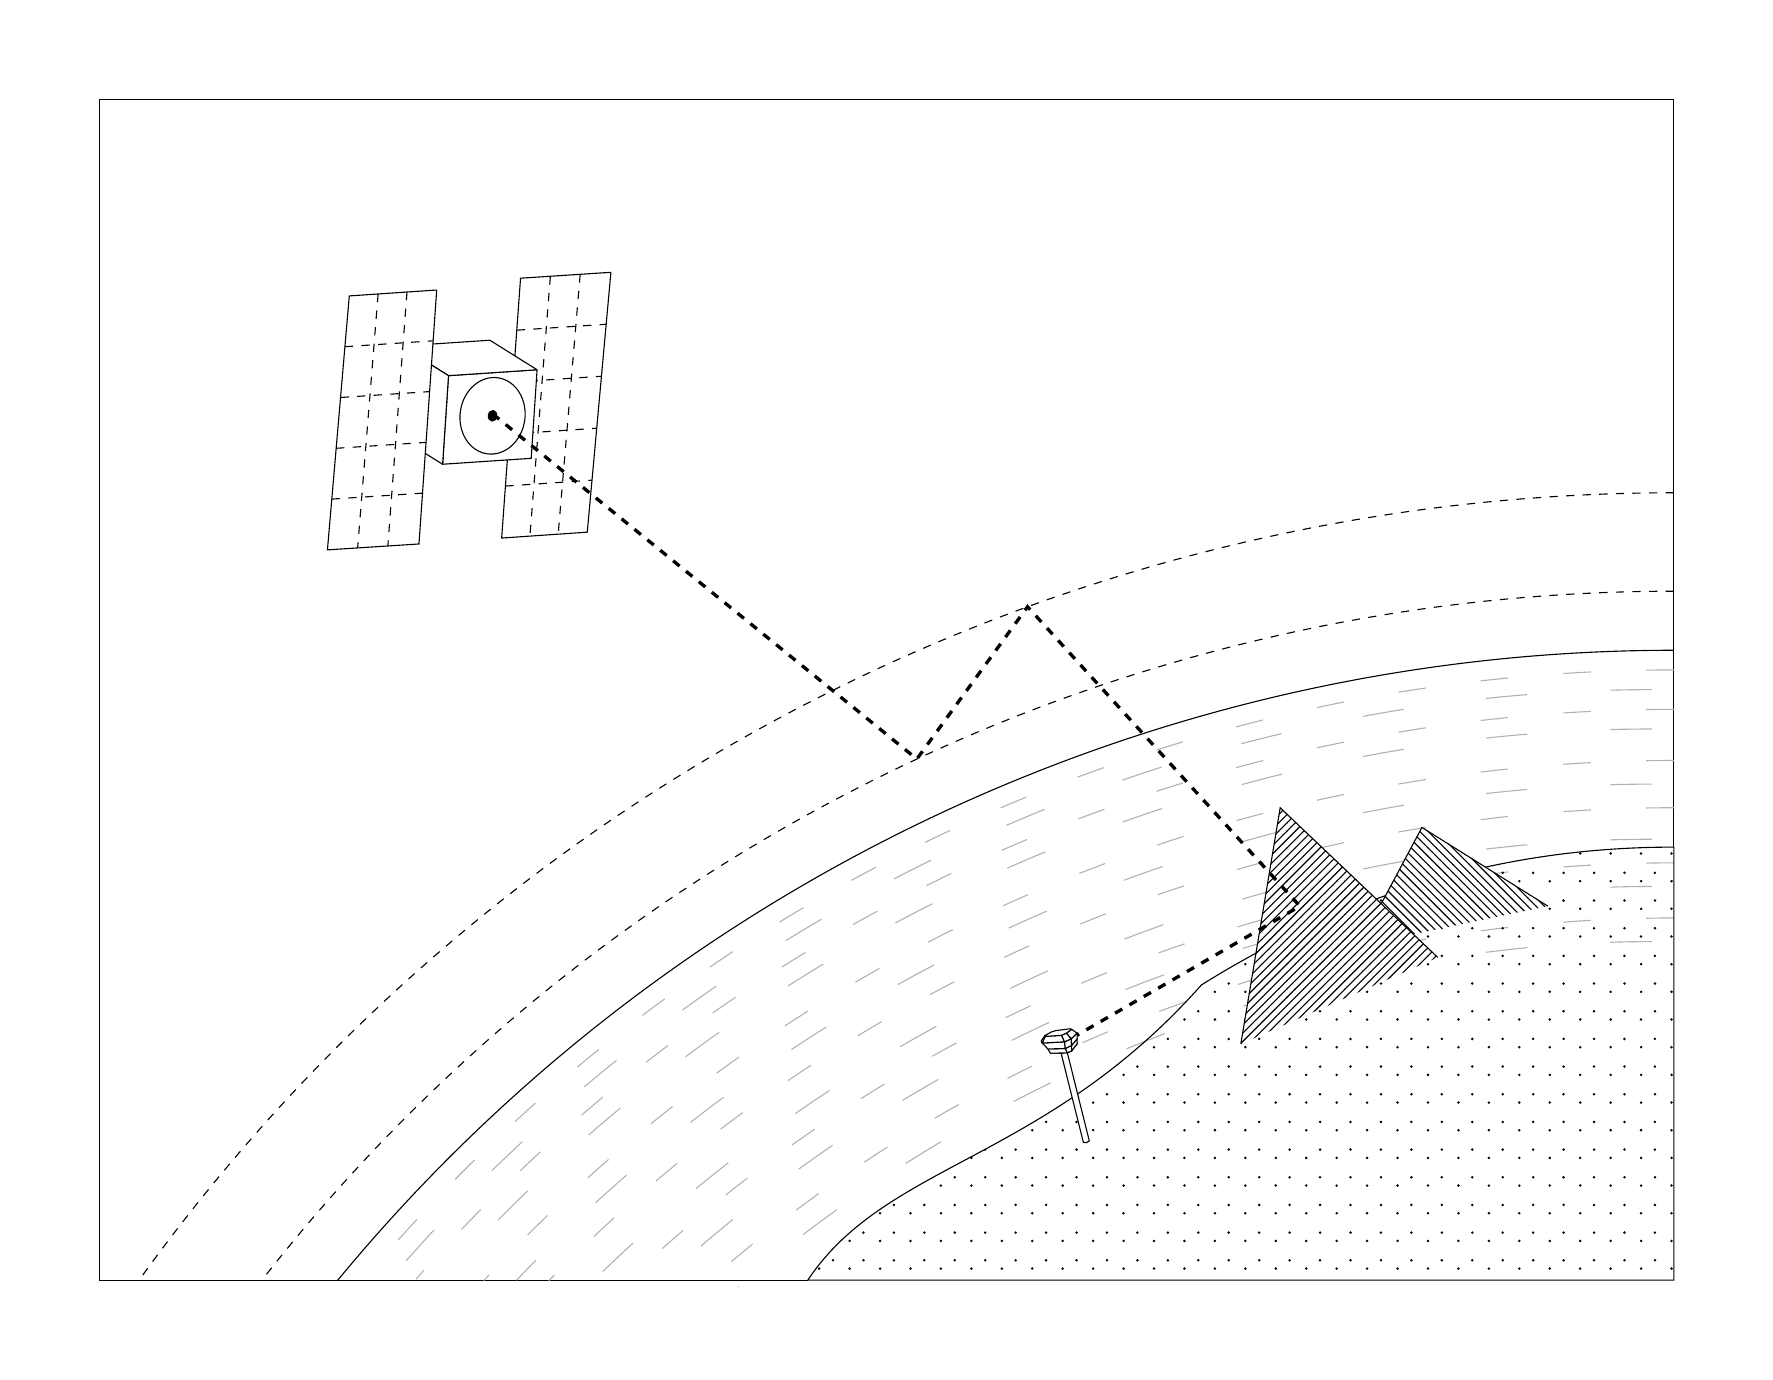
\begin{tikzpicture}[domain=0:20,samples=300]
  \begin{pgfonlayer}{foreground}
    % Mountains
    \coordinate (rm_left) at (16,4.25);
    \coordinate (rm_top) at (16.8,5.75);
    \coordinate (rm_right) at (18.4,4.75);
    
    \draw[fill=white,draw opacity=0] (rm_left) -- (rm_top) -- (rm_right);
    \draw[pattern=north west lines] (rm_left) -- (rm_top) -- (rm_right);
    
    \coordinate (lm_left) at (14.5,3);
    \coordinate (lm_top) at (15,6);
    \coordinate (lm_right) at (17,4.1);
    
    \draw[fill=white,draw opacity=0] (lm_left) -- (lm_top) -- (lm_right);
    \draw[pattern=north east lines] (lm_left) -- (lm_top) -- (lm_right);
    
    \coordinate (sat) at (5,11);
    \path (sat) pic[scale=0.75] {satellite};
    
    \coordinate (rcv) at (12.5,1.75);    
    \coordinate (earth_center) at (20,-14);
    
    \coordinate (s0) at (sat);
    \coordinate (_s1) at (20,8.75); \coordinate (s1) at ([rotate around={25:(earth_center)}] _s1);
    \coordinate (_s2) at (20,10); \coordinate (s2) at ([rotate around={20:(earth_center)}] _s2);
    \coordinate (s3) at ($ (lm_top) + (0.25,-1.25) $);
    \coordinate (s4) at ($ (rcv) + (-0.1,1.35) $);
    
    \draw[very thick,dashed] (s0) -- (s1) -- (s2) -- (s3) -- (s4);
    
    \path (rcv) pic[scale=0.6,rotate=14] {receiver};
  \end{pgfonlayer}
  
  \begin{pgfonlayer}{background}
    % \draw[step=1cm,black,thin,opacity=0.2,dashed] (20.9,-0.9) grid (-0.9,15.9);
    \draw[opacity=0] (20.9,-0.9) grid (-0.9,15.9);
    
    \draw (9,0) -- (0,0) -- (0,15) -- (20,15) -- (20,5.5);
    
    \draw (20,8) arc (90:140.5:22cm);
    \draw[dashed] (20,8.75) arc (90:142:22.75cm);
    \draw[dashed] (20,10) arc (90:144.2:24cm);
    
    \draw[gray!60,dash pattern=on 10pt off 20pt] (20,7.75) arc (90:140:21.75cm);
    \draw[gray!60,dash pattern=on 15pt off 30pt,shorten <=8] (20,7.5) arc (90:140.5:21.5cm);
    \draw[gray!60,dash pattern=on 10pt off 20pt] (20,7.25) arc (90:138.75:21.25cm);
    \draw[gray!60,dash pattern=on 15pt off 30pt,shorten <=8] (20,7) arc (90:137.5:21cm);
    \draw[gray!60,dash pattern=on 10pt off 20pt] (20,6.6) arc (90:137.2:20.6cm);
    \draw[gray!60,dash pattern=on 15pt off 30pt,shorten <=8] (20,6.3) arc (90:136.4:20.3cm);
    \draw[gray!60,dash pattern=on 10pt off 20pt] (20,6) arc (90:135.6:20cm);
    \draw[gray!60,dash pattern=on 15pt off 30pt,shorten <=8] (20,5.6) arc (90:135:19.6cm);
    \draw[gray!60,dash pattern=on 10pt off 20pt] (20,5.3) arc (90:133.5:19.3cm);
    \draw[gray!60,dash pattern=on 15pt off 30pt,shorten <=8] (20,5) arc (90:133:19cm);
    \draw[gray!60,dash pattern=on 10pt off 20pt] (20,4.6) arc (90:132:18.6cm);
    \draw[gray!60,dash pattern=on 15pt off 30pt,shorten <=8] (20,4.3) arc (90:130.5:18.3cm);
    
    \draw[pattern=my crosshatch dots] 
      (9,0) -- (20,0) -- (20,5.5) .. controls (18,5.5) and (16,5) .. (14,3.75) .. controls (12,1.5) and (10,1.5) .. (9,0);
  \end{pgfonlayer}
\end{tikzpicture}
\end{document}